\section{Brugere og opgaver}

De to vigtigste opgaver som prototypen skal understøtte er beskrevet i de
følgende afsnit.

\subsection{Oprettelse af medlemsskab}

Oprettelse af medlemsskab er en væsentlig del af Pensionistsagens hjemmeside.
Det er gennem dette medlemsskab at folk kan få attraktive rabatter og tilbud
på en lang række ting i hjemmesidens tilhørende webshop.

Idet en væsentlig del af hjemmesidens brugergruppe udgør personer med kun
ringe IT-kyndighed jf. PACT-analysen fra \cite{opgave2} er det vigtigt at
denne process er så simpel som muligt, samt at man let er i stand til at
finde tilmeldingssiden. Opgaven minder meget om scenariet ``Tilmelding til
Pensionistsagen'' fra \cite{opgave2} hvor Karl Koder hjælper et familiemedlem
med at tilmelde sig. Opgaven skal dog også være i stand til at blive løst
af en pensionist alene såfremt denne besider basale færdigheder om brug af
internettet.

Den kontekstuelle undersøgelse fra \cite{opgave3} gav ikke anledning til at
tilmeldingssiden skulle ændres i nogen væsentlig grad.

\subsubsection{Udførsel af opgaven}

Fra forsiden på Figur~\ref{fig:opg1_trin1} klikker brugeren på
linket ``Medlemsservice'' i undermenuen hvorefter han får vist
skærmbilledet i Figur~\ref{fig:opg1_trin2} og udfylder formularen som vist
i Figur~\ref{fig:opg1_trin3}. Når brugeren har klikket på ``Fuldfør
tilmelding''-knappen bliver han mødt med en side der kort fortæller at
tilmeldingen lykkedes som i Figur~\ref{fig:opg1_trin4}.

% {{{ screenshots
\begin{figure}[h]
    \centering
    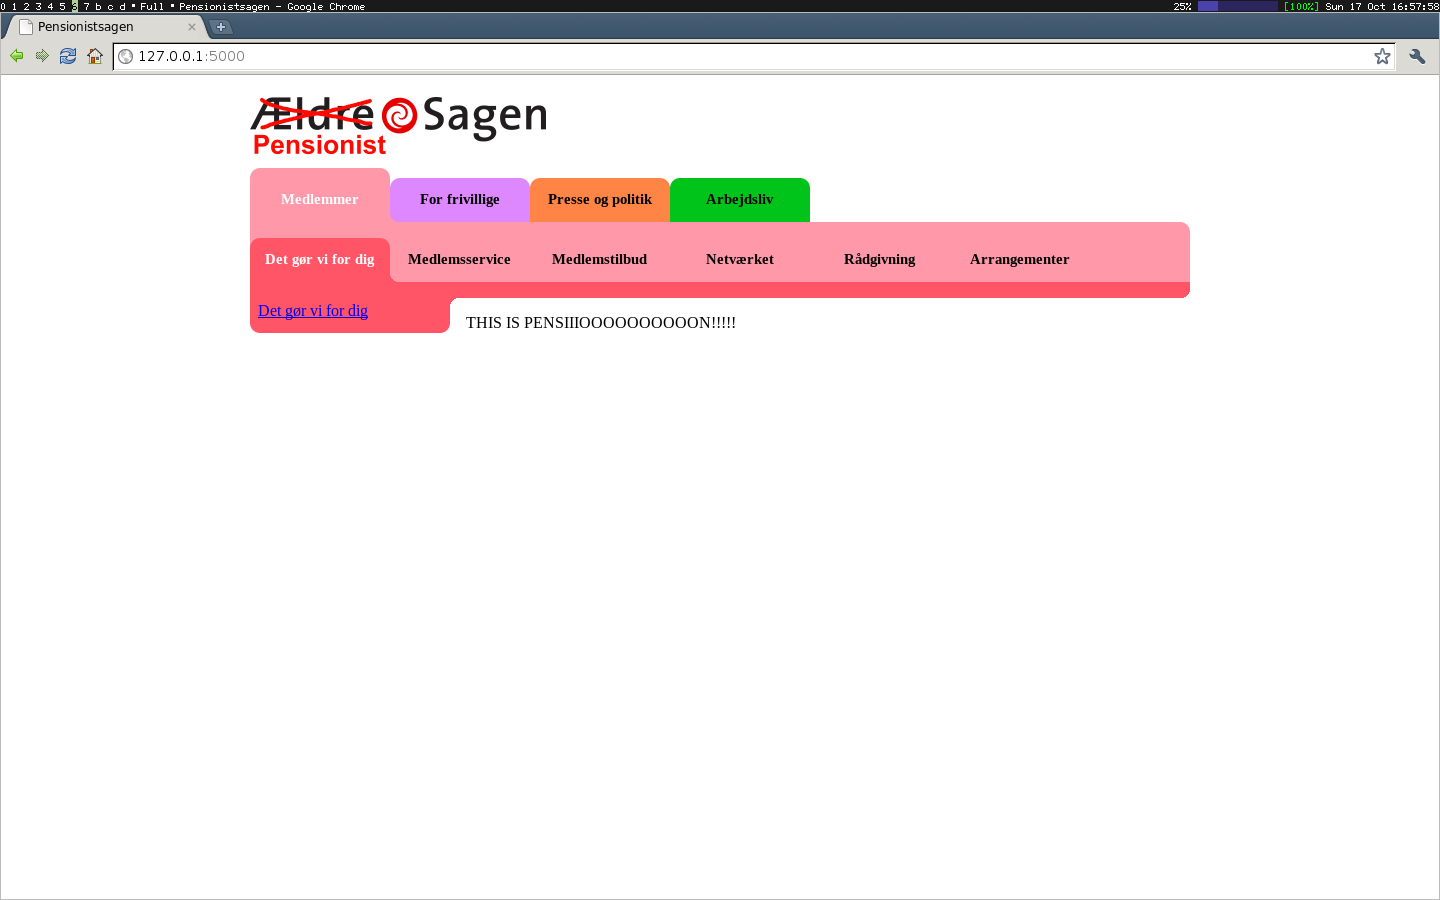
\includegraphics[width=.95\textwidth]{billeder/opgave1_trin1.png}
    \caption{Pensionistsagens forside. Indeholder i prototypen ikke nogen relevant information.}
    \label{fig:opg1_trin1}
\end{figure}
\begin{figure}[h]
    \centering
    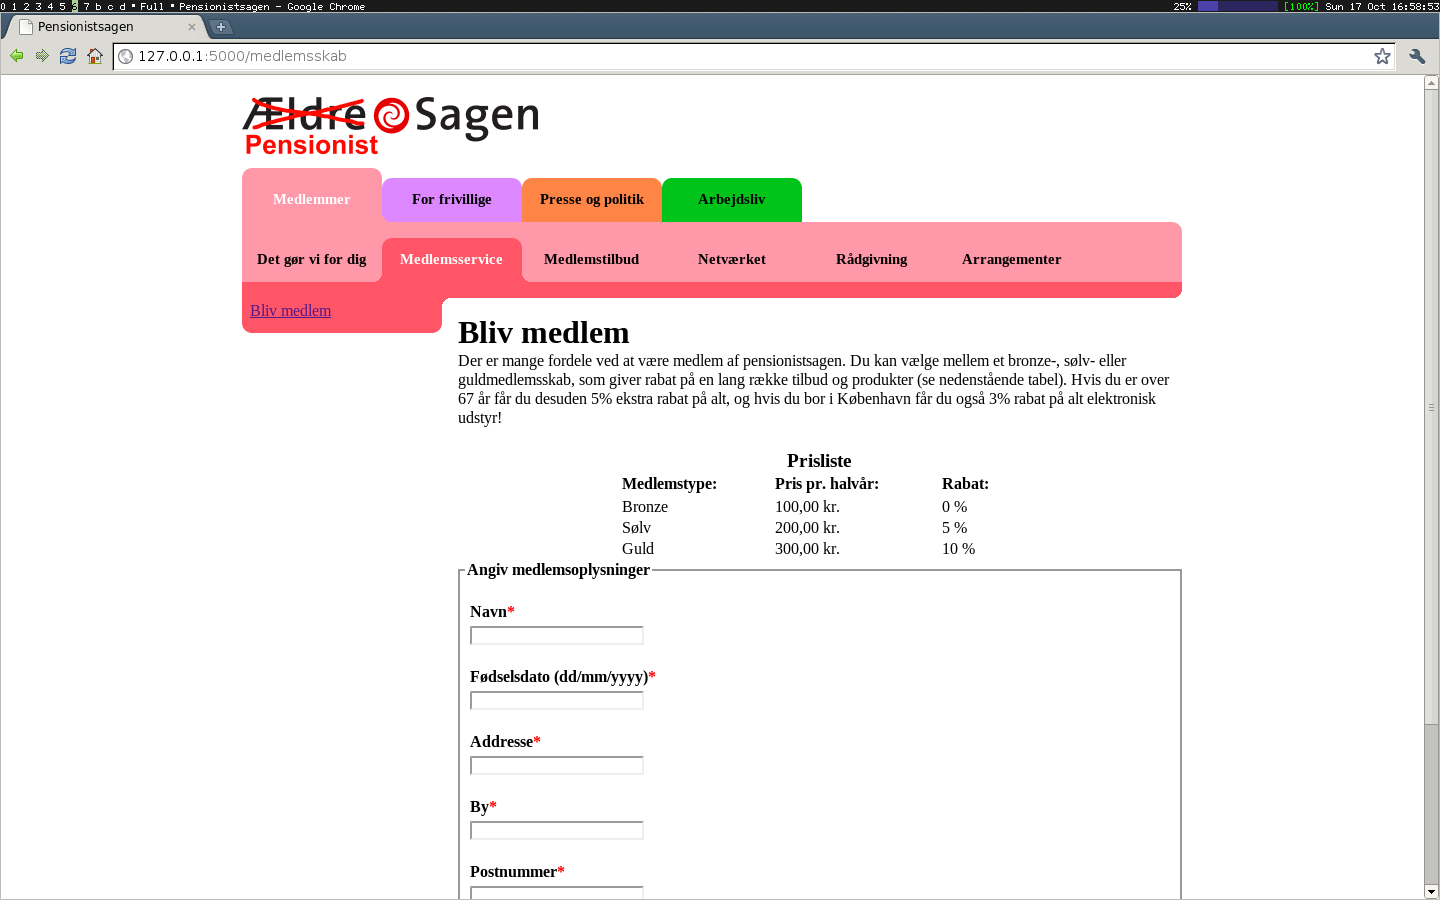
\includegraphics[width=.95\textwidth]{billeder/opgave1_trin2.png}
    \caption{Forsiden for ``Bliv medlem''. Brugeren kan her se en forklarende tekst om de forskellige medlemstyper, se en oversigt i tabellen samt udfylde personlige informationer.}
    \label{fig:opg1_trin2}
\end{figure}
\begin{figure}[h]
    \centering
    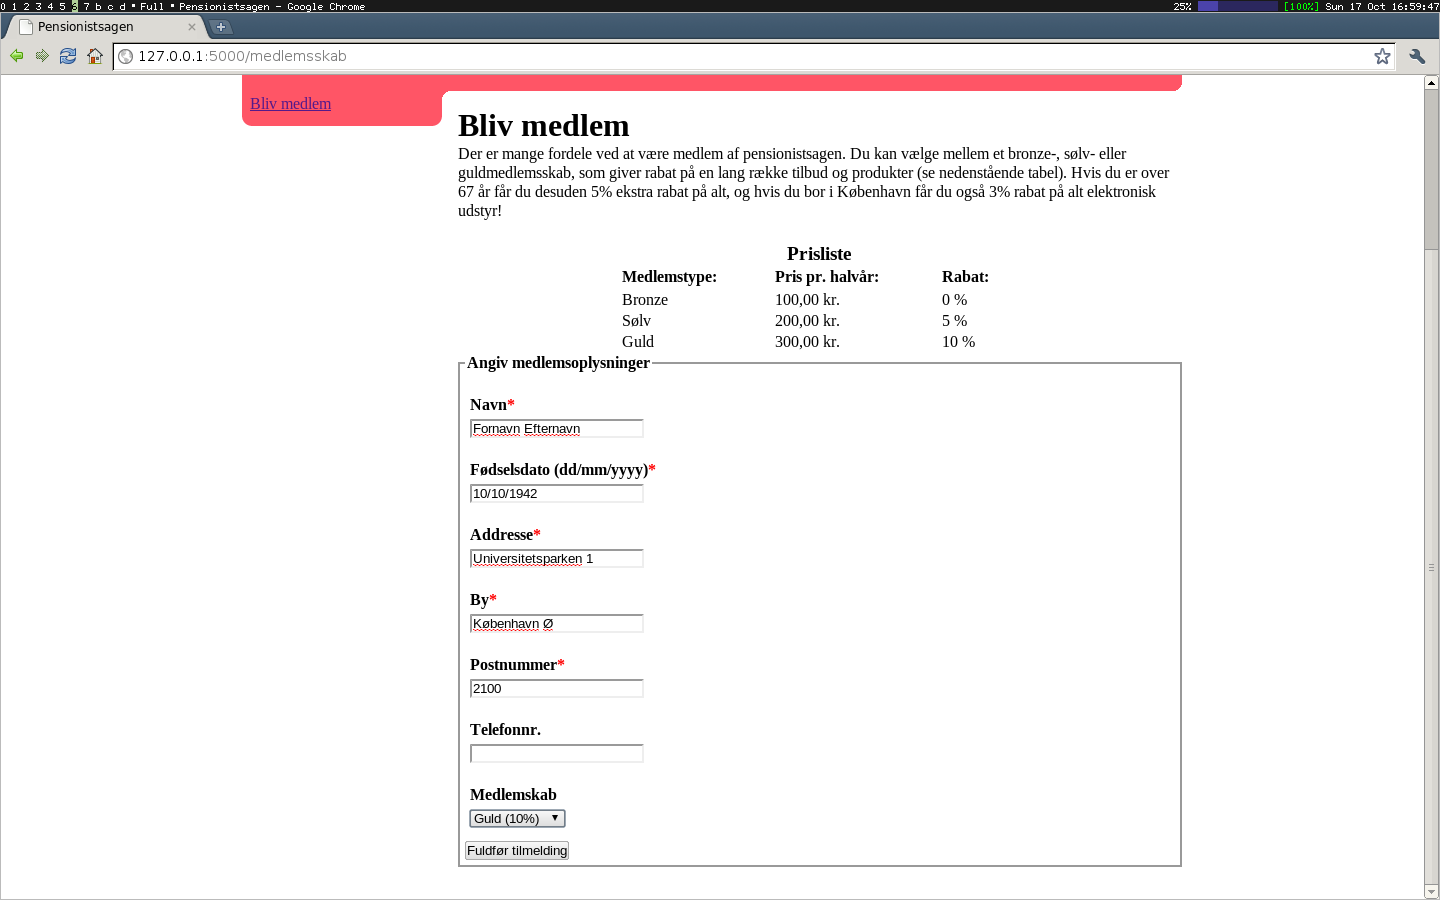
\includegraphics[width=.95\textwidth]{billeder/opgave1_trin3.png}
    \caption{Felterne i formularen er blevet udfyldt.}
    \label{fig:opg1_trin3}
\end{figure}
\begin{figure}[h]
    \centering
    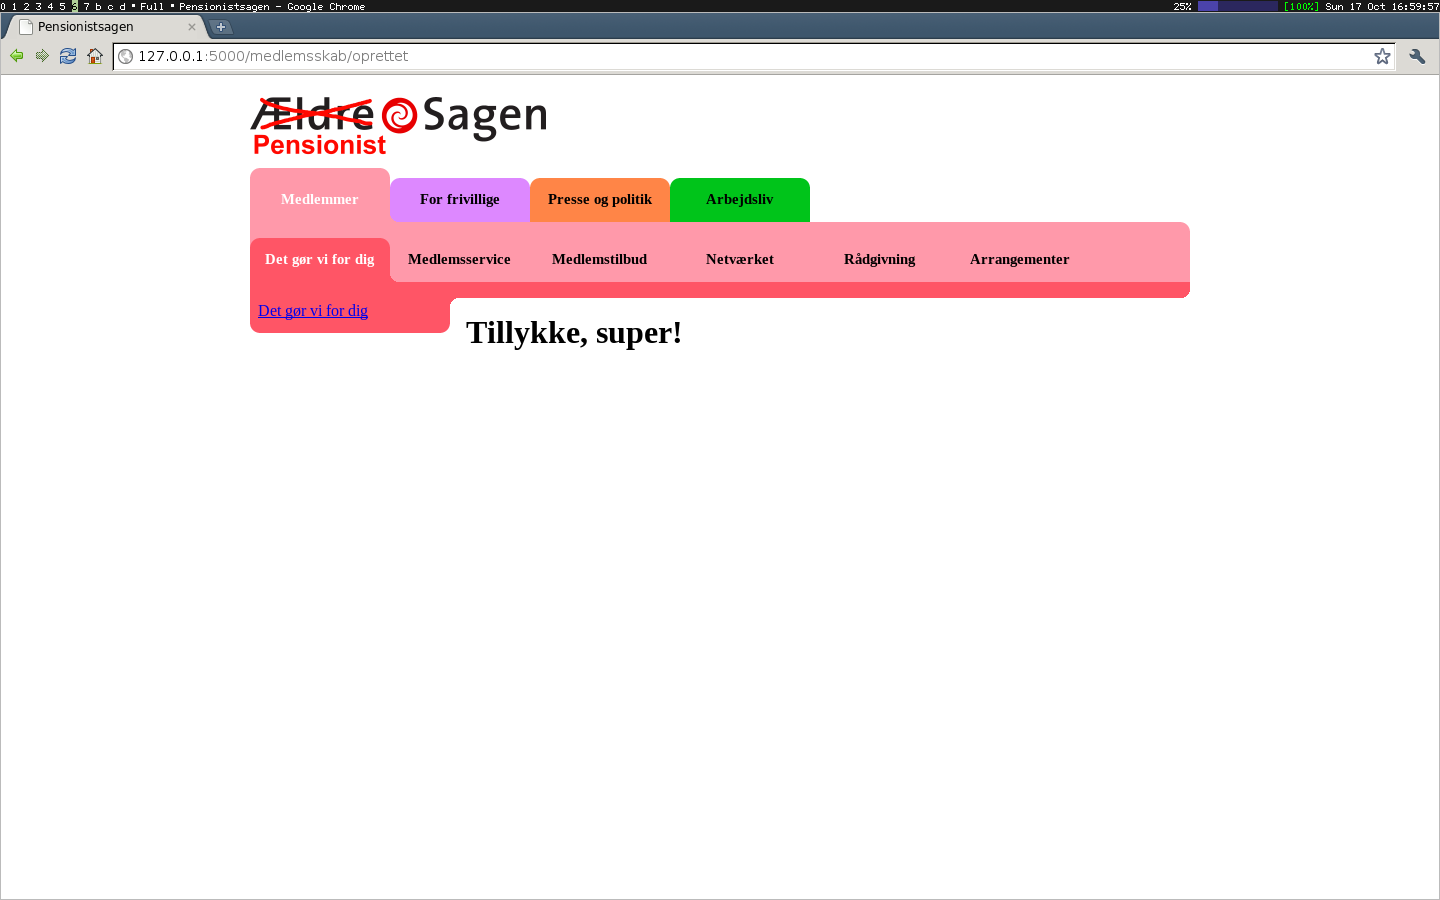
\includegraphics[width=.95\textwidth]{billeder/opgave1_trin4.png}
    \caption{Formularen er blevet udfyldt og sendt.}
    \label{fig:opg1_trin4}
\end{figure}
% }}}

\subsection{Køb af tilbud/varer}

En anden vigtig del af Pensionistsagens hjemmeside er webshopdelen hvor
brugeren kan købe forskellige produkter samt billeter til diverse
arrangementer.

Som i forrige brugeropgave fremkommer de samme problemstillinger fra
PACT-analysen i \cite{opgave2}. I den kontekstuelle undersøgelse fra
\cite{opgave3} fremkom der en forvirring om hvor man kunne finde ting som
koncerter. Folk søgte inde under både ``Medlemstilbud'' og ``Arrangementer''
efter disse. Denne problemstilling har vi valgt at imødekomme ved at lade
begge sektioner af hjemmesiden vise disse, men på forskellige måder.
Førstnævnte har en kategorisk visning, mens sidstnævnte har en kronologisk
visning i form af en kalender. Et andet problem var at man ikke kunne finde
information om transport o.l. til arrangementer, men dette løses forholdsvist
let ved at skrive en ordentlig produktbeskrivelse, og prototypen behøves
således ikke at ændres af den grund.

\subsubsection{Udførsel af opgave}

Fra forsiden af Pensionistsagens hjemmeside (Figur~\ref{fig:opg2_trin1})
klikker brugeren på ``Arrangementer'' i menuen. Herefter lander man på
arrangementsiden hvor man kan se en oversigt over de kommende arrangementer
i kalenderen (Figur~\ref{fig:opg2_trin2}). Fra kalenderen kan et arrangement
vælges, og i Figur~\ref{fig:opg2_trin3} er ``Violinkoncert (Brahms)''
blevet valgt hvor brugeren så kan se produktbeskrivelse, video fra en
tidligere koncert samt kommentarer fra andre brugere (sidstnævnte ikke
synligt i Figur~\ref{fig:opg2_trin3}). Efter klik på ``Køb''-knappen
bliver brugeren ledt gennem købsprocessen bestående af leveringsadresse
(Figur~\ref{fig:opg2_trin4}), betalingsform (Figur~\ref{fig:opg2_trin5}) og
til sidst bekræftelse af købet (Figur~\ref{fig:opg2_trin6}).

% {{{ screenshots
\begin{figure}[h]
    \centering
    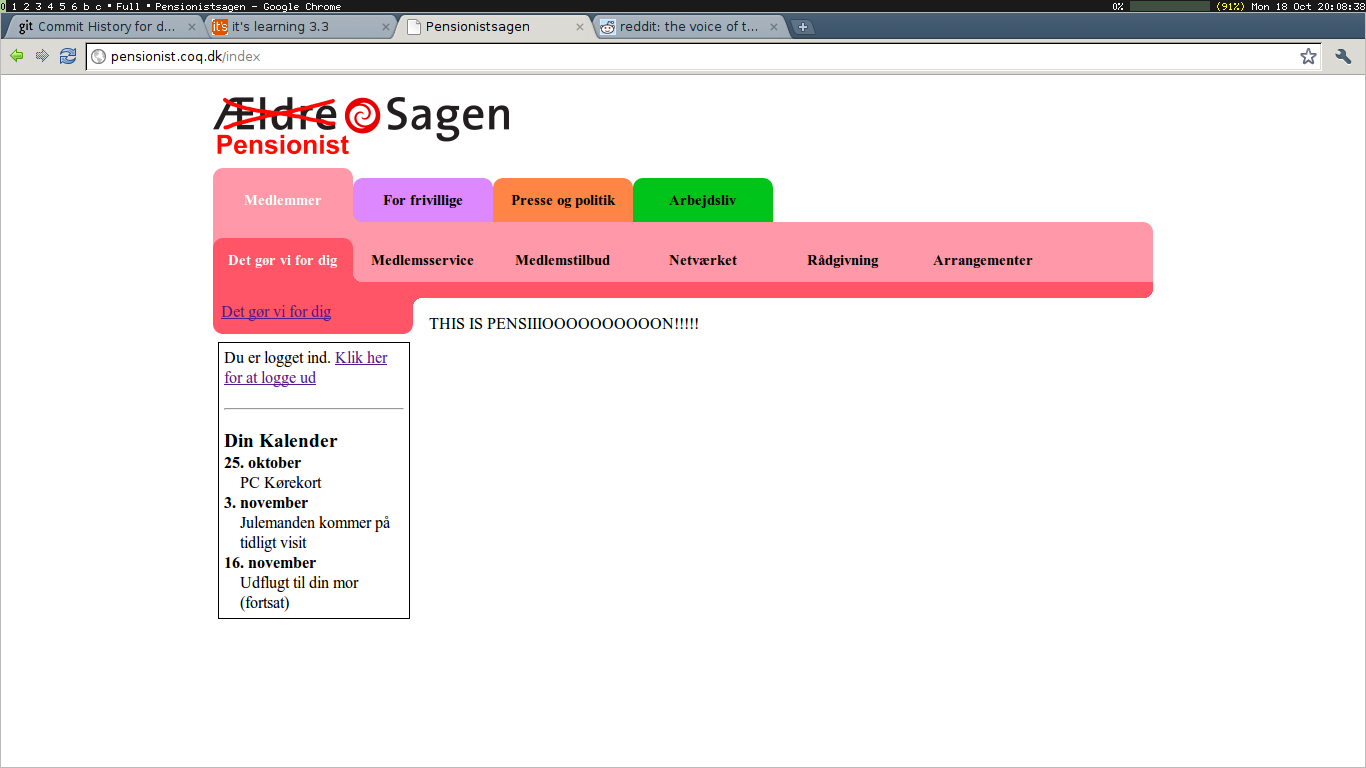
\includegraphics[width=.95\textwidth]{billeder/opgave2_trin1.png}
    \caption{Pensionistsagens forside en bruger der er logget ind.}
    \label{fig:opg2_trin1}
\end{figure}
\begin{figure}[h]
    \centering
    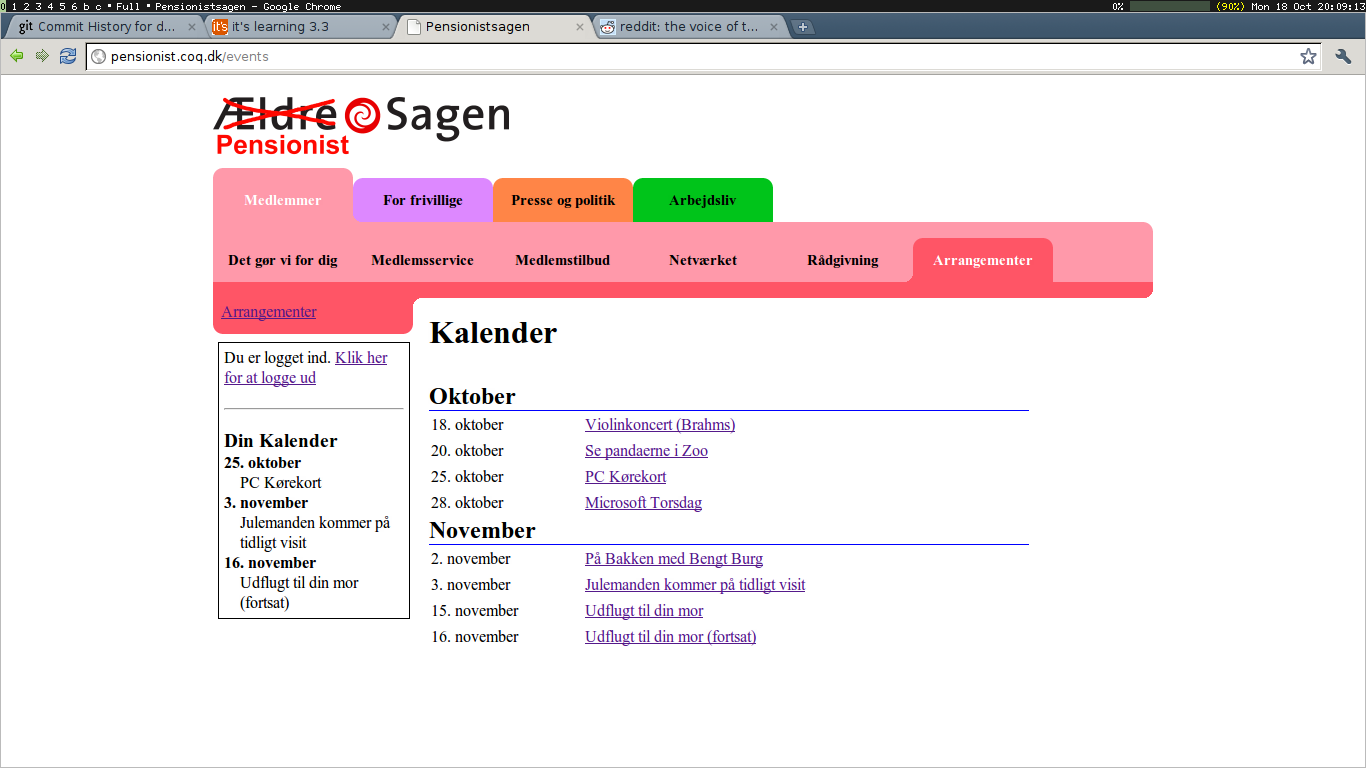
\includegraphics[width=.95\textwidth]{billeder/opgave2_trin2.png}
    \caption{Kalender over kommende arrangementer.}
    \label{fig:opg2_trin2}
\end{figure}
\begin{figure}[h]
    \centering
    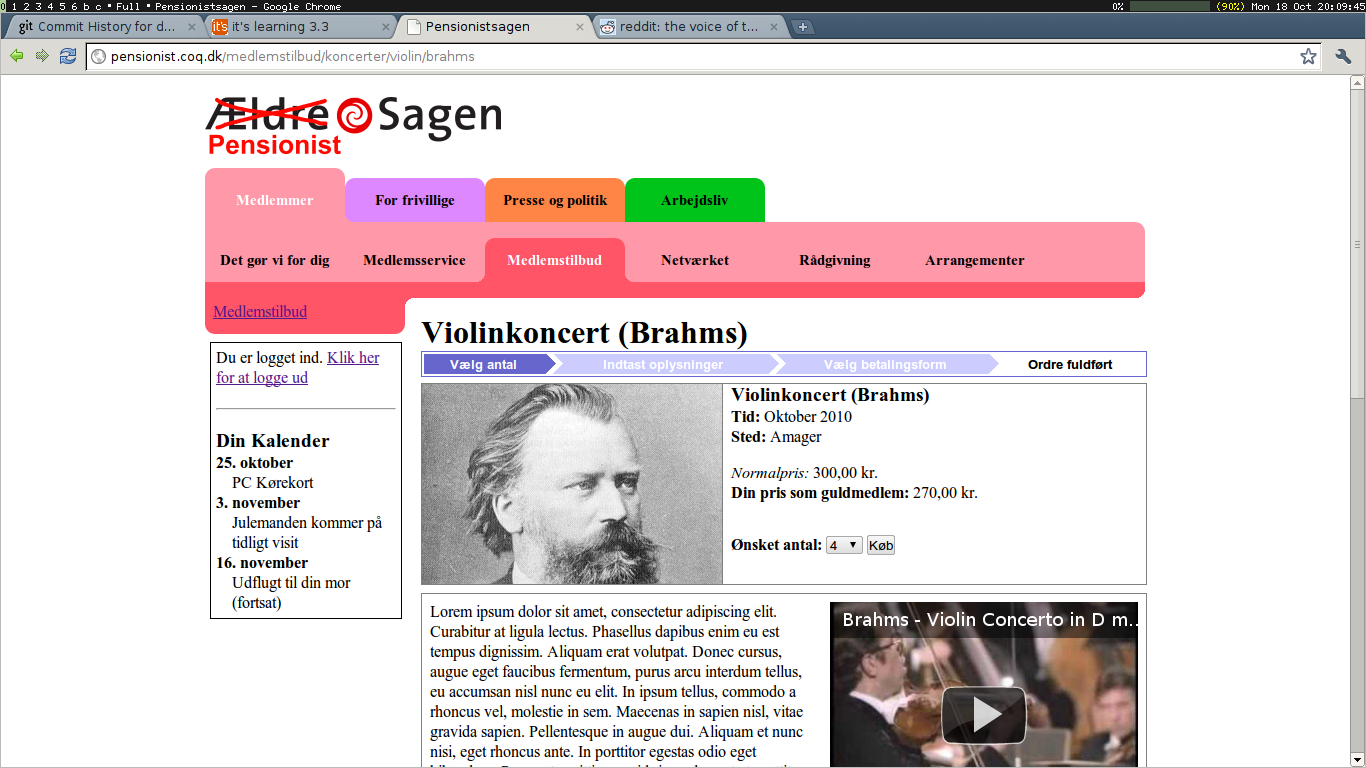
\includegraphics[width=.95\textwidth]{billeder/opgave2_trin3.png}
    \caption{Købssiden indeholdende bl.a. produktbeskrivelse for en koncert.}
    \label{fig:opg2_trin3}
\end{figure}
\begin{figure}[h]
    \centering
    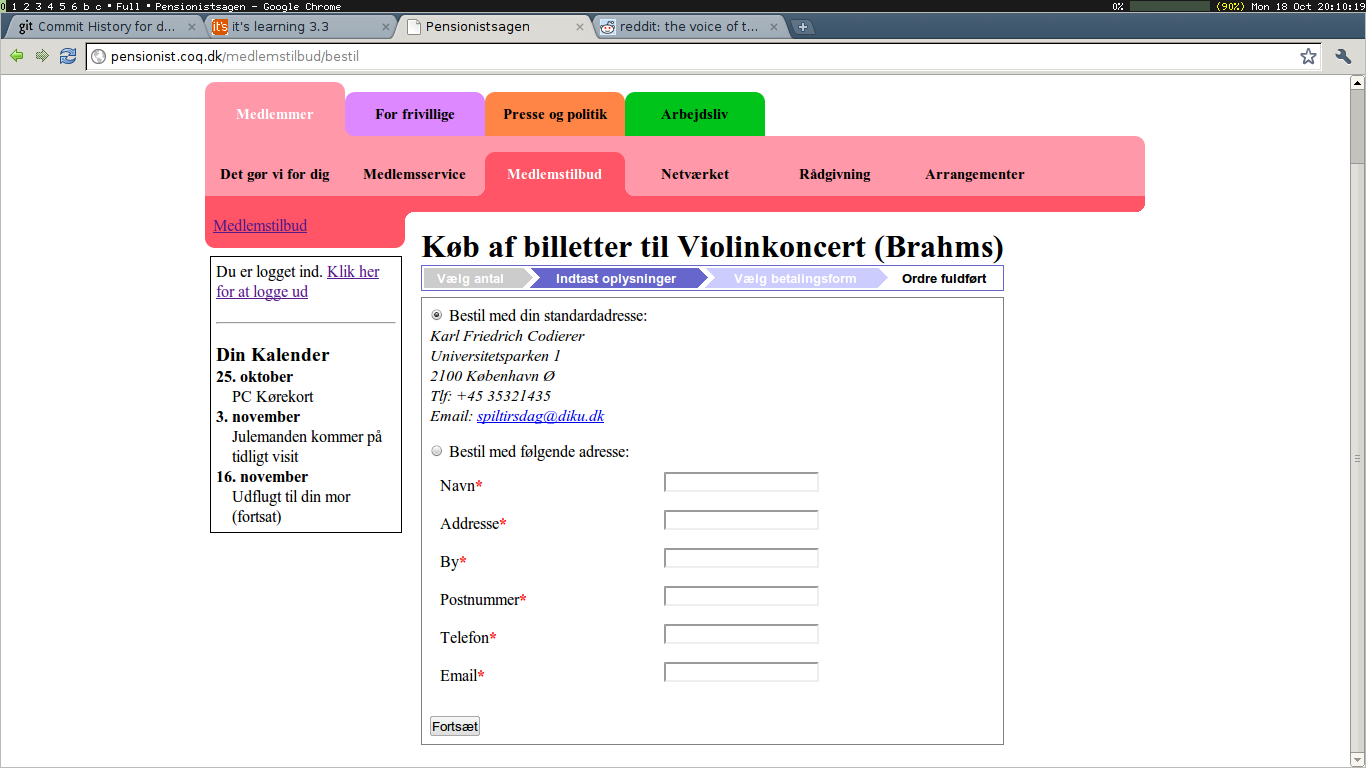
\includegraphics[width=.95\textwidth]{billeder/opgave2_trin4.png}
    \caption{Indtastning af leveringsadresse ved køb.}
    \label{fig:opg2_trin4}
\end{figure}
\begin{figure}[h]
    \centering
    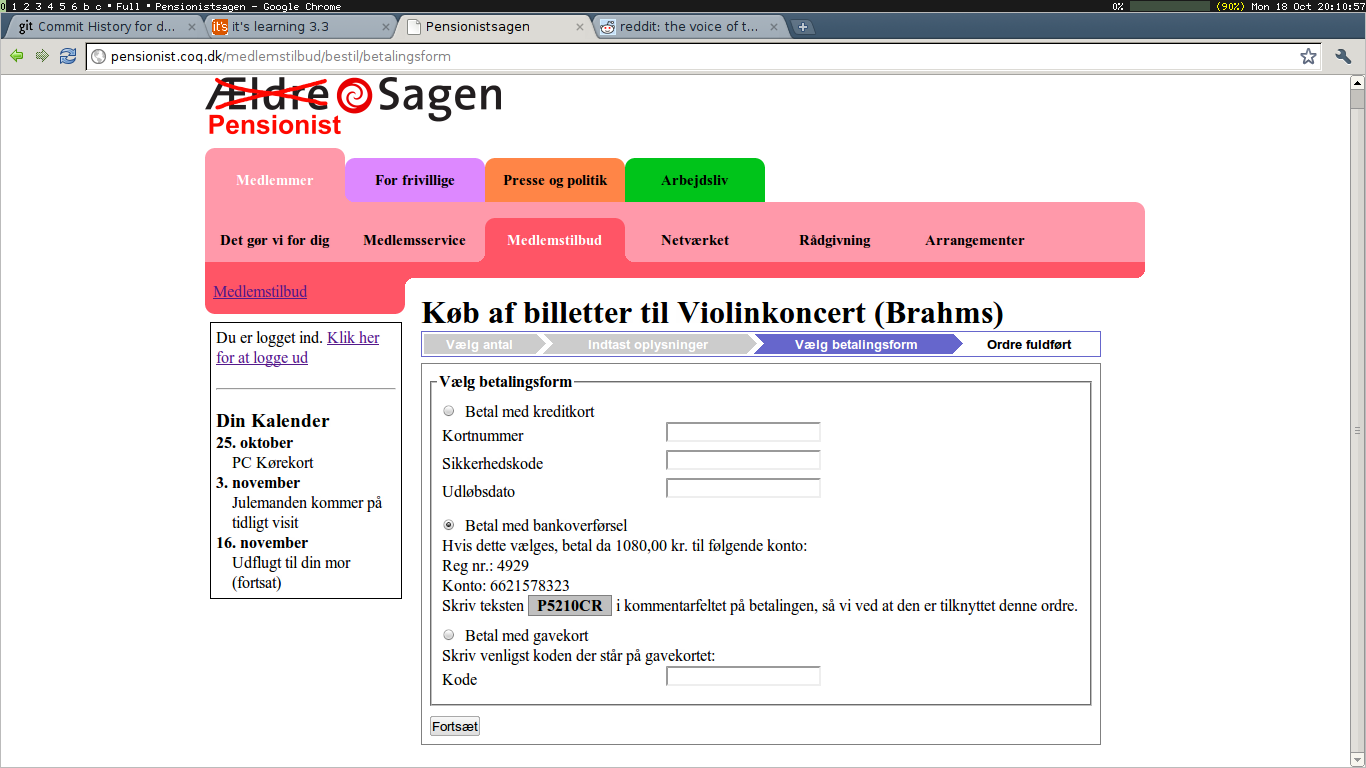
\includegraphics[width=.95\textwidth]{billeder/opgave2_trin5.png}
    \caption{Valg af betalingsform ved køb.}
    \label{fig:opg2_trin5}
\end{figure}
\begin{figure}[h]
    \centering
    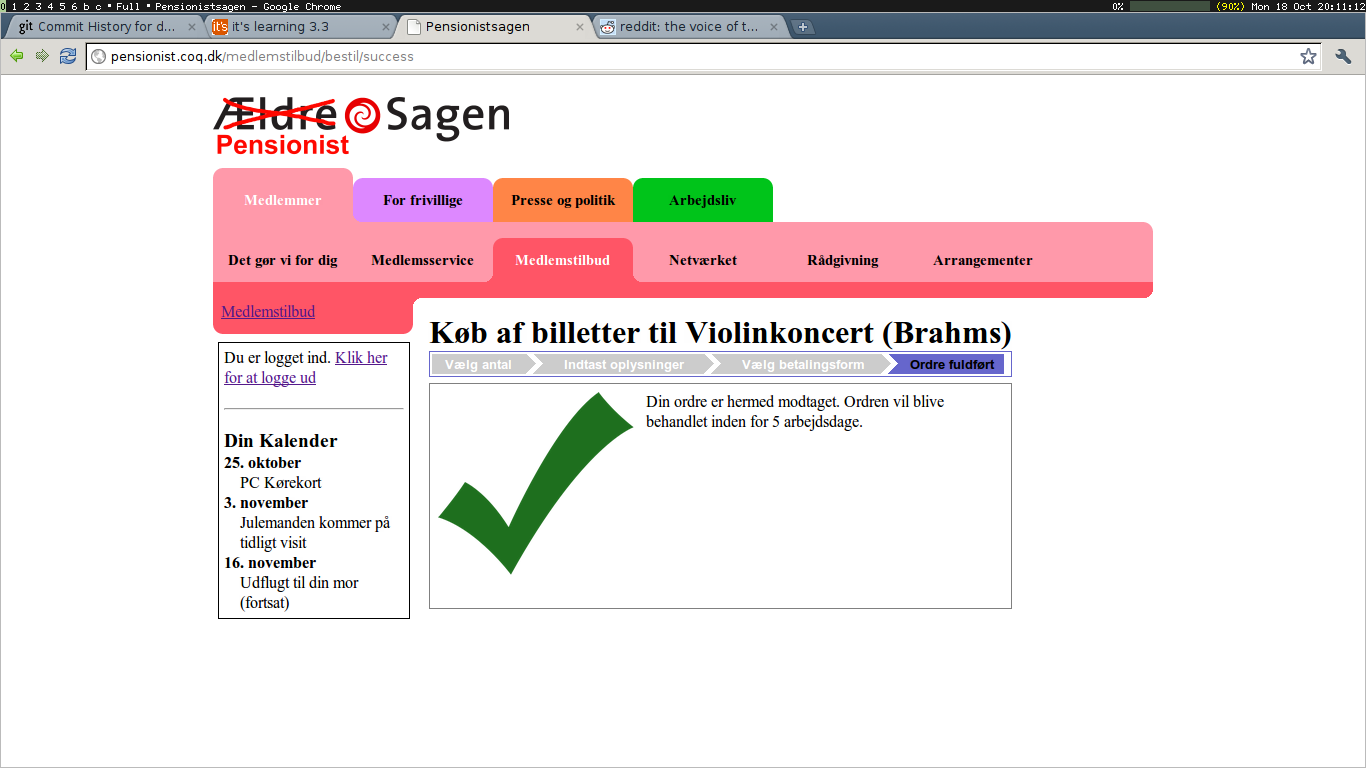
\includegraphics[width=.95\textwidth]{billeder/opgave2_trin6.png}
    \caption{Bekræftelse af køb efter købsprocessen er fuldendt.}
    \label{fig:opg2_trin6}
\end{figure}
% }}}
